% !Mode:: "TeX:UTF-8"
% VL 9, gebaut aus part-representation-learning/15-variational-autoencoder.md
% und 16-word2vec.md. Die fünf Graphen-Rahmen sind am 2026-11-04 nach
% parkplatz-vl14-graphen.tex ausgezogen, weil der Plan die Graphen in VL 14 führt.
% (Dialogmuster: transcripts/vl08-vae-word2vec-2025 und vl09-representation-learning-2025).
% !Mode:: "TeX:UTF-8"
\newcommand{\thepage}{} % to silence a hyperref warning about pdfpagelabels
\RequirePackage[]{silence}
\WarningsOff[hyperref]
\PassOptionsToPackage{log-declarations=false}{xparse}
%\RequirePackage[l2tabu, orthodox]{nag}
\RequirePackage{luatex85} % to make \pdf...= commands work with LuaTeX
\documentclass[aspectratio=169,t]{beamer}
\usepackage{ifthen}
\usepackage[T1]{fontenc}
\usepackage{iftex}
% `no-math` ist nicht optional. Ohne die Option übernimmt fontspec die Mathe-Schrift
% teilweise: Operatoren, Ziffern, Klammern und Funktionsnamen wie \tanh kommen dann aus
% Source Sans 3, die Variablen weiter aus Computer Modern -- zwei Schriftbilder in
% einer Formel, dasselbe Übel wie in PLAYBOOK-folien.md §2.3, nur eine Ebene tiefer.
% Sichtbar wurde es am 2026-10-21 an \Longrightarrow: Der Pfeil wird aus \Relbar und
% \Rightarrow zusammengesetzt, das `=` kam aus Source Sans 3 und der Schaft aus CMSY,
% die Balken trafen sich nicht, und der Pfeil fiel auseinander. Mit `no-math` kommt das
% `=` aus CMR und alles passt. Gegenprobe: pdffonts an einem formelreichen Deck.
% Seit dem 2026-11-04 **Source Sans 3**, nicht mehr Source Sans Pro: Adobe hat die
% Familie 2021 umbenannt und zaehlt die Hauptversion seither im Namen mit (zuletzt
% 3.052, 2023-04). Der Name ist der Familienname, nach dem fontspec sucht -- unter dem
% alten Namen findet es die alte 2.021. Debian trixie hat sie als
% `fonts-adobe-sourcesans3` (3.052+dfsg), lokal liegt dieselbe Fassung als OTF in
% ~/.fonts/SourceSans3. Beides SIL OFL, also auch im CI-Image mitlieferbar.
\ifLuaTeX
 \usepackage[no-math]{fontspec}
 \setmainfont[Ligatures=TeX]{Source Sans 3}
\else
 \usepackage[utf8]{inputenc}
\fi
% Sprache: Bis zum 2026-10-02 stand hier das veraltete german.sty. Es sucht \l@german,
% findet es im LuaTeX-Format nicht und meldet "\language number for German undefined,
% default 255 used": kein Deck trennte deutsche Silben. Jetzt babel wie im tex-Template
% des Buchs, shorthands=off, damit das Anführungszeichen nicht aktiv wird. LuaTeX lädt
% die Trennmuster beim ersten Gebrauch aus hyph-utf8 (im Log: "German Hyphenation
% Patterns (Reformed Orthography, 2006)"); fehlen sie, warnt babel ("No hyphenation
% patterns were preloaded for the language 'ngerman'") und trennt ebenfalls nicht.
\usepackage[shorthands=off,ngerman]{babel}
\usepackage{newunicodechar}
\newunicodechar{€}{\texteuro}
\newunicodechar{ß}{\ss}
\renewcommand{\SS}{\iffontchar\font"1E9E \symbol{"1E9E}\else SS\fi}
\usepackage{ellipsis}
\usepackage{microtype}
\usepackage{listings}
\usepackage{sourcecodepro}
\lstset{language=Python, basicstyle=\ttfamily}
\usepackage{amsfonts}
\usepackage{amssymb}
\usepackage{amsthm}
\usepackage{tabularx} % für \optionen (Antwortgitter der mitmachfrage)
\usepackage{fancyhdr}
\usepackage{graphicx}

\newtheorem{proposition}[theorem]{Proposition}

\DeclareMathOperator*{\argmax}{argmax}
\DeclareMathOperator{\supp}{supp}
\newcommand{\E}{\ensuremath{\mathbb{E}}}
\newcommand{\V}{\ensuremath{\mathbb{V}}}

% Hervorhebungen in der Markenfarbe des Buchs (BRANDING.md), nicht in xcolor-purple.
% Das Theme bleibt HHU-Blau; die Markenfarbe ist nur der Akzent.
\definecolor{eidlbrand}{HTML}{6F59A6}
\setbeamercolor{emph}{fg=eidlbrand}
\renewcommand<>{\emph}[1]{%
  {\usebeamercolor[fg]{emph}\only#2{\itshape}#1}%
}

% --- Mitmachfrage (Peer Instruction): Kasten mit Frage und Optionen, danach \pause und
%     \antwort mit Begründung. Übernommen am 2026-10-14 aus ds2-26 (`ds2figures.tex`),
%     wo sich das Format bewährt hat; absichtlich zeilengleich, damit die Kursfamilie
%     nicht auseinanderläuft (PLAYBOOK-folien.md §2.1).
%     \begin{mitmachfrage}[Titel] ... \end{mitmachfrage}
\setbeamercolor{mitmachtitel}{fg=white,bg=hhuorange}
\setbeamercolor{mitmachkoerper}{fg=black,bg=hhuorange!8}
\newenvironment{mitmachfrage}[1][Frage an Sie]{%
  \begin{beamerboxesrounded}[upper=mitmachtitel,lower=mitmachkoerper,shadow=false]{#1\hfill
    {\normalfont\tiny Aufzeichnung: anhalten, selbst antworten}}}{%
  \end{beamerboxesrounded}}
\newcommand{\antwort}{\textcolor{hhuorange}{\textbf{Antwort:}}\ }

% --- Antwortoptionen als 2x2-Gitter statt als Fließtext mit \quad und \\.
%     Eingeführt 2026-10-14: Im Fließtext richten sich A--D nicht aneinander aus, der
%     Umbruch hängt an der Länge der vorigen Option, und bei vier langen Optionen sieht
%     die Folie zerfasert aus. Das Gitter gibt feste Spalten und gleiche Grundlinien.
%     \optionen{...}{...}{...}{...}  -- immer genau vier, in der Reihenfolge A B C D.
\newcommand{\optlabel}[1]{\textcolor{hhuorange}{\textbf{#1}}\,}
%     Das Gitter steht eine Stufe kleiner als der Fragetext: Es sind Wahlmöglichkeiten,
%     keine Aussagen, und bei vier langen Optionen liefe der Rahmen sonst über (am
%     2026-10-14 an den drei Lesetext-Folien von VL 1 gemessen, 6 bis 14 pt).
\newcommand{\optionen}[4]{%
  \par\smallskip
  {\small
  \begin{tabularx}{\linewidth}{@{}>{\raggedright\arraybackslash}X@{\hspace{1.5em}}>{\raggedright\arraybackslash}X@{}}
    \optlabel{A} #1 & \optlabel{B} #2\\[4pt]
    \optlabel{C} #3 & \optlabel{D} #4
  \end{tabularx}\par}}

% --- Marker im Folientitel für klausurnahe Stellen:
%     \frametitle{Die Google-Matrix\pruefungsfrage}
\newcommand{\pruefungsfrage}{%
  \ \raisebox{1.5pt}{\rotatebox{3}{\colorbox{hhuorange}{%
    \textcolor{white}{\normalfont\tiny\bfseries Gute Prüfungsfrage}}}}}



\hypersetup{draft=false,colorlinks=false,pdfpagemode=UseOutlines,plainpages=false,
            breaklinks=true,bookmarksnumbered=true,pdfborder=0 0 0,
            pdftitle={Einführung in Deep Learning WiSe 2026/27 HHU},
            pdfauthor={Konrad Voelkel},
            pdfsubject={deep learning}}

%\documentclass[aspectratio=169,t]{beamer}
\usetheme{hhubeamer} % put the hhu-beamer-theme in /usr/share/texmf/tex/latex/beamer/themes/

% Folientitel: Das Theme setzt den Titel als tikz-Knoten ohne Breitenbegrenzung, lange Titel
% laufen unter das Logo. Dieselbe Vorlage wie in beamerinnerthemehhubeamer.sty, nur mit
% text width, sodass ein zu langer Titel vor dem Logo umbricht statt darunter zu laufen.
% Das Theme wählt die Vorlage "hhubeamer" vor jedem Frame neu, deshalb wird sie hier unter
% demselben Namen ersetzt (defbeamertemplate verweigert sonst die Neudefinition).
\makeatletter
\expandafter\let\csname beamer@@tmpop@frametitle@hhubeamer\endcsname\@undefined
\defbeamertemplate{frametitle}{hhubeamer}[1][]
{%
\ifnum\value{page}>1%
  \begin{beamercolorbox}[wd=\paperwidth,ht=2.11cm]{frametitle}
    \begin{tikzpicture}
      \useasboundingbox[fill=white](0,0) rectangle(\the\paperwidth,2.11);
      \ifx\insertframetitle\@empty%
      \else%
        \fill[hhublue] (0,1.5) rectangle ++(0.3,-0.5);
        \fill[hhublue] (0.3,1.25) circle (0.25);
        \draw[hhuiceblue!65,thick] (.9,0.4) -- ++(12,0);
      \fi
      \node[anchor=south] at (14.5,-.02) {\includegraphics[height=16.8mm]{fig/template/HHU-vertikal.pdf}};
      \ifx\insertframesubtitle\@empty%
          {\node[anchor=west, hhublue,font=\LARGE, text width=12.4cm, align=left] at (.75,1.22){\insertframetitle};}
      \else%
          {\node[anchor=west, hhublue,font=\LARGE, text width=12.4cm, align=left] at (.75,1.22){\insertframetitle};
          \node[anchor=west, hhublue,font=\large] at (.75,0){\insertframesubtitle};}%
      \fi
    \end{tikzpicture}
  \end{beamercolorbox}
  \ifx\insertframetitle\@empty%
    \vspace{-1.5cm}
  \fi
\fi
}
\makeatother

% Schrift: Das Theme lädt helvet (Type-1-Familie phv). Unter LuaTeX/fontspec gibt es die in der
% TU-Kodierung nicht ("Font shape TU/phv undefined"), und LaTeX fiel still auf Latin Modern Roman
% zurück. Beamer setzt in der Sans-Familie, deshalb hier \setsansfont, und zwar *nach* dem Theme.
% professionalfonts lässt die Mathe-Fonts in Ruhe (Latin Modern Math, kursive Variablen), statt
% sie wie Beamers Standard-Fonttheme serifenlos und aufrecht zu verbiegen.
\usefonttheme{professionalfonts}
\ifLuaTeX
  \setsansfont[Ligatures=TeX]{Source Sans 3}
\fi

% Notizseite (Deck mit `show notes on second screen=right`): Beamer paginiert Notizen
% nicht. Mit dem Standard-Layout (Vorschaubild der Folie oben) passte die Titelnotiz von
% VL 1 (Ablaufplan plus Kürzungsregeln) nicht auf die Seite und brach mitten im Satz ab.
% Ohne Vorschaubild und in \scriptsize passt sie (Befund A5 der Durchsicht vom 2026-09-25,
% umgesetzt 2026-10-02). Auf die Folien selbst hat das keine Wirkung.
\setbeamertemplate{note page}[plain]
\setbeamerfont{note page}{size=\scriptsize}

% -------------------- Code listings config --------------------
% Define custom colors for syntax highlighting
\definecolor{codegreen}{rgb}{0,0.6,0}
\definecolor{codegray}{rgb}{0.5,0.5,0.5}
\definecolor{codepurple}{rgb}{0.58,0,0.82}
\definecolor{backcolour}{rgb}{0.96,0.96,0.94} % Very light gray/beige
% Configure the listings package
\lstset{
    language=Python,
    backgroundcolor=\color{backcolour},   
    commentstyle=\color{codegreen}\itshape,
    keywordstyle=\color{blue}\bfseries,
    numberstyle=\tiny\color{codegray},
    stringstyle=\color{codepurple},
    basicstyle=\ttfamily\footnotesize, % Use a monospaced font
    breakatwhitespace=false,         
    breaklines=true,      
             % Enable automatic line breaking
    captionpos=b,                      % Caption at the bottom
    keepspaces=true,                 
    numbers=left,                      % Line numbers on the left
    numbersep=10pt,                    % Distance of line numbers from the code
    showspaces=false,                
    showstringspaces=false,            % Don't show weird underscores in strings
    showtabs=false,                  
    tabsize=4,
    frame=single,                      % Add a subtle border around the code
    rulecolor=\color{black!20},        % Border color
  }

\event[]{}
\author[Wintersemester 2026/27]{Dr. Konrad Völkel, Wintersemester 2026/27}

%\title{Data Science, VL 1}
%\date{16.04.2026}


%%% Local Variables:
%%% mode: latex
%%% TeX-master: t
%%% End:


% Fassung mit Dozentennotizen (zweiter Schirm): die nächste Zeile einkommentieren.
% \setbeameroption{show notes on second screen=right}

\graphicspath{{../images/}}

\title[VAE und word2vec (VL 9)]{VAE und word2vec\\\large Einführung in Deep Learning, VL 9}
\date{09.12.2026}

\begin{document}

\begin{frame}
  \titlepage

  \note{\textbf{Ablauf, 90 Minuten.} Zwei Kapitel. Die Graphen sind am 2026-11-04 nach
    VL 14 gerückt, direkt vor das Empfehlungssystem -- die knapp 26 Minuten, die sie hier
    hatten, gehen an den VAE und an die Fragerunde:\\[2pt]
    \begin{tabular}{@{}rll@{}}
      0--8   & Folie 2       & Rückblick Autoencoder, Löcher im latenten Raum\\
      8--22  & Folien 3--5   & Rauschen dazu, der Reparametrisierungstrick\\
      22--38 & Folien 6--8   & VAE-Training, KL-Term, Recap\\
      38--48 & Folien 9--10  & word2vec: Ziel und Kernidee\\
      48--60 & Folien 11--12 & CBOW und Skip-gram\\
      60--72 & Folien 13--14 & Token statt Wörter, Dokumente vergleichen\\
      72--80 & Folie 15      & Übungsblatt\\
      80--90 & Reserve       & Fragen, und der KL-Term in Ruhe\\
    \end{tabular}\\[4pt]
    2025 gab es nach dem VAE eine siebenminütige Fragerunde -- die Zeit ist jetzt da,
    der Reparametrisierungstrick braucht sie. Und beim KL-Term aufpassen: 2025 wurde in
    der Sitzung begründet, Sigma \emph{explodiere}, im Skript steht die umgekehrte
    Richtung (Sigma geht gegen null). Das Skript hat recht.}
\end{frame}

\begin{frame}
  \frametitle{Das Problem mit dem latenten Raum}

  \begin{center}
    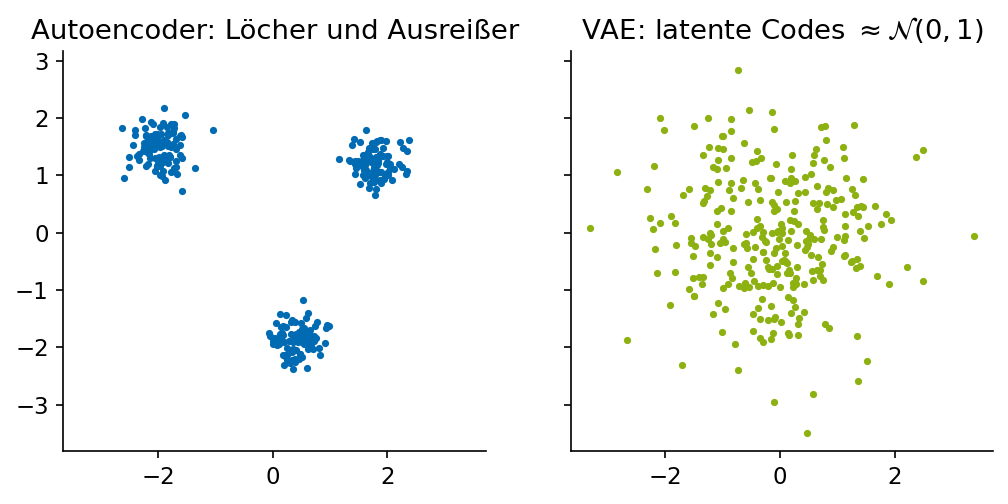
\includegraphics[width=0.62\textwidth]{vl08-latent-300points.png}
  \end{center}

  \note{300 Datenpunkte im latenten Raum eines klassischen Autoencoders: Löcher und
    Ausreißer.
    Frage in den Raum: Was passiert, wenn ich an einer Stelle dekodiere, an der kein
    Datenpunkt liegt? Antwort: Matsch. Genau das wollen wir reparieren -- wir hätten
    gern einen Raum, in dem man \emph{überall} dekodieren kann.}
\end{frame}

\begin{frame}
  \frametitle{Die Idee: Rauschen dazu}

  \begin{center}
    \Large
    Auch $\operatorname{MSE}\bigl(x, \operatorname{dec}(\operatorname{enc}(x) + \varepsilon)\bigr)$
    soll klein sein.
  \end{center}

  \bigskip
  \begin{center}
    \normalsize Der Decoder muss eine ganze \emph{Umgebung} auf $x$ abbilden.
  \end{center}

  \note{Aus jedem Punkt wird eine Wolke. Der latente Raum wird glatt.
    Sofort die Frage stellen, die kommen muss: \emph{Wie geht Backpropagation durch ein
    Sampling?} Antwort: $\varepsilon$ hängt nicht von den Gewichten ab, ist im
    Rückwärtsdurchlauf also eine Konstante -- ganz normale Kettenregel.
    Das ist die Stelle, an der 2025 die meisten Fragen kamen.}
\end{frame}

\begin{frame}
  \frametitle{Drei Punkte, drei Wolken}

  \begin{center}
    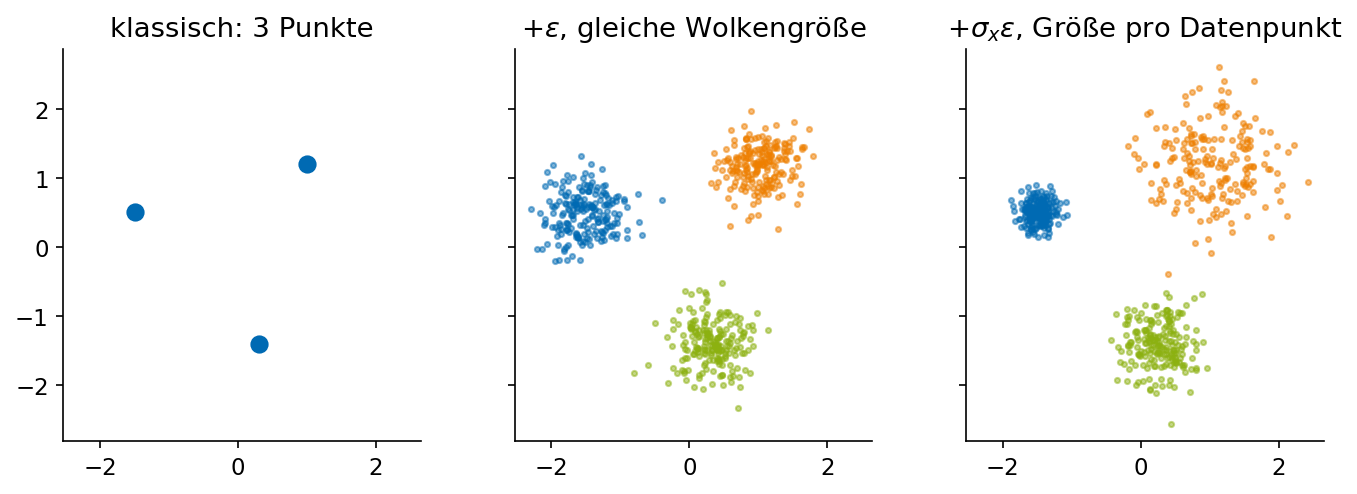
\includegraphics[width=0.78\textwidth]{vl08-latent-3points.png}
  \end{center}

  \note{Links klassisch: drei Punkte. Mitte: mit gleichem Rauschen $+\varepsilon$ --
    drei gleich große Wolken. Rechts: mit datenabhängigem $\sigma_x$ -- die Wolkengröße
    wird pro Datenpunkt gelernt.
    Das dritte Bild ist der VAE.}
\end{frame}

\begin{frame}
  \frametitle{Der Reparametrisierungstrick}

  \begin{center}
    \Large
    Problem: $\varepsilon \sim \mathcal{N}(0, \sigma_x^2)$ -- $\sigma_x$ hängt an den Gewichten.\\[16pt]
    \Huge $y = \mu_x + \sigma_x\,\varepsilon$, \quad $\varepsilon \sim \mathcal{N}(0,1)$
  \end{center}

  \note{Aus einer Verteilung zu sampeln, deren \emph{Parameter} von den Gewichten
    abhängen, lässt sich nicht ableiten. Nach dem Umschreiben ist $\varepsilon$ wieder
    eine Konstante und $\sigma_x$ ein ganz normaler Ausgang des Encoders, durch den
    Gradienten fließen.
    Das ist die Stelle, an der der VAE steht und fällt -- langsam machen, notfalls an
    der Tafel.}
\end{frame}

\begin{frame}
  \frametitle{VAE-Training}

  \begin{center}
    \Large
    Encoder liefert $2L$ Ausgänge: $\mu_x$ und $\sigma_x$\\[14pt]
    $L_{\text{VAE}} = \operatorname{MSE}(x, \operatorname{dec}(y))
      + D_{KL}\bigl(q(y\mid x)\,\|\,\mathcal{N}(0,1)\bigr)$
  \end{center}

  \note{Ohne KL-Term hat das Training zwei Ausreden: $\sigma_x \to 0$ lernen (dann ist es
    wieder ein klassischer Autoencoder) oder $\mu_x$ explodieren lassen (dann liegen die
    Wolken weit auseinander und der Raum füllt sich nie).
    \textbf{Wichtige Feinheit:} Die beiden $\mathcal{N}(0,1)$ sind \emph{nicht} dasselbe!
    Das erste ist die Rauschquelle, das zweite die Prior-Verteilung, an die sich die
    latenten Verteilungen anschmiegen sollen.
    In der Praxis gibt der Encoder \texttt{logvar} aus, damit kein Ausgang auf positive
    Werte eingeschränkt werden muss.}
\end{frame}

\begin{frame}
  \frametitle{Der KL-Term, geschlossen}

  \begin{center}
    \Huge $D_{KL} = \tfrac12\bigl(\mu^2 + \sigma^2 - 1 - \ln\sigma^2\bigr)$
  \end{center}

  \bigskip
  \begin{center}
    \normalsize Das ist genau der negative ELBO aus Data Science.
  \end{center}

  \note{Für Normalverteilungen gibt es die geschlossene Form -- deshalb ist der Term
    billig.
    Wer nach dem Zusammenhang zu EM fragt: Ein GMM fittet \emph{wenige} Cluster und ordnet
    jeden Punkt einem zu. Der VAE geht umgekehrt vor -- \emph{jeder} Datenpunkt bekommt
    seine eigene Normalverteilung, und der KL-Term sorgt dafür, dass alle zusammen
    ungefähr eine Standardnormalverteilung ergeben.}
\end{frame}

\begin{frame}
  \frametitle{VAE im Bild}

  \begin{center}
    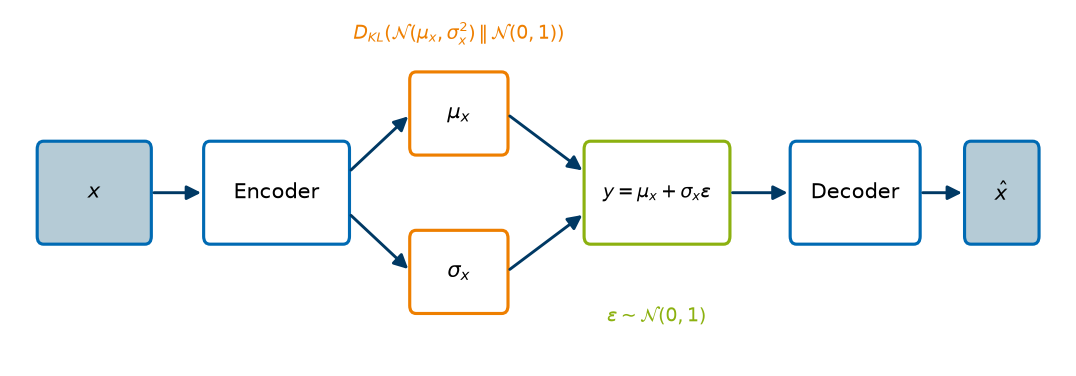
\includegraphics[width=0.66\textwidth]{vl08-vae-schema.png}
  \end{center}

  \note{Recap: Encoder gibt eine Normalverteilung aus, Decoder rekonstruiert aus einer
    Stichprobe, Loss ist Rekonstruktion plus KL zum Prior.
    Und dann kann man \emph{generieren}: $y \sim \mathcal{N}(0,1)$ sampeln und dekodieren.
    VAEs stecken heute noch in Bildgeneratoren -- bei Stable Diffusion findet die
    Diffusion im latenten Raum eines VAE statt.}
\end{frame}

% ------------------------------------------------------------------ word2vec
\begin{frame}
  \frametitle{Dieselbe Idee für Text}

  \begin{center}
    \Large
    Wörter $\longrightarrow$ Vektoren,\\[10pt]
    sodass ähnliche Wörter nah beieinander liegen.
  \end{center}

  \note{One-Hot-Vektoren sind alle gleich weit voneinander entfernt -- ein Autoencoder
    darauf lernt nichts über Bedeutung. Das ist der Punkt, an dem word2vec ansetzt.
    Vorverarbeitung: zählen, Stopwords raus, die häufigsten $N$ (etwa 5000) behalten,
    One-Hot kodieren, und eine Abbildung $\mathbb{R}^N \to \mathbb{R}^K$ mit $K \approx 200$
    suchen.}
\end{frame}

\begin{frame}
  \frametitle{Die Kernidee}

  \begin{center}
    \Large „Die [MASK] frisst ihr Futter am liebsten aus dem goldenen Napf.“
  \end{center}

  \bigskip
  \begin{center}
    \normalsize Die Bedeutung eines Wortes ergibt sich aus seiner Verwendung.
  \end{center}

  \note{Distributional hypothesis. Der Task ist ein Denoising Autoencoder, bei dem das
    Rauschen im \emph{Löschen} eines Wortes besteht -- die Brücke zu letzter Woche
    ausdrücklich schlagen. Und zu Fill-Mask aus VL 3.
    Den Hörsaal raten lassen, was [MASK] ist: Katze, Hündin -- und genau deshalb liegen
    die beiden im latenten Raum nah beieinander.}
\end{frame}

\begin{frame}
  \frametitle{CBOW und Skip-gram}

  \begin{center}
    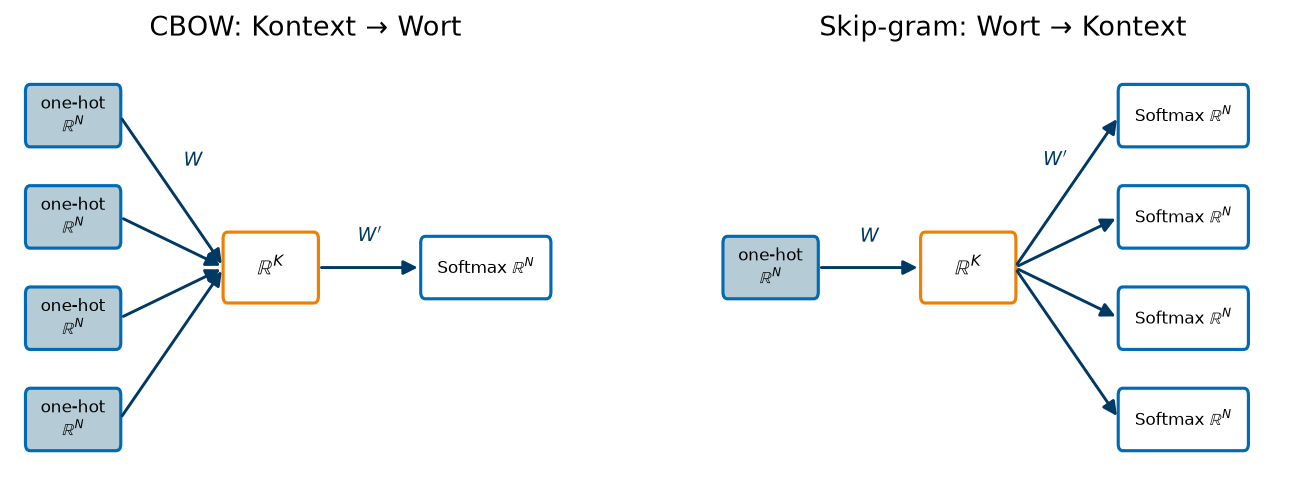
\includegraphics[width=0.72\textwidth]{vl08-cbow-skipgram.png}
  \end{center}

  \note{Zwei Matrizen: $W$ (Encoder, $N \to K$) und $W'$ (Decoder, $K \to N$).
    CBOW: aus $2S$ Kontextwörtern das mittlere vorhersagen. Skip-gram: umgekehrt.
    Loss ist jeweils NLL gegen den One-Hot-Vektor.}
\end{frame}

\begin{frame}
  \frametitle{Wo sind die Wortvektoren?}

  \begin{center}
    \Huge $e(w) = W w$
  \end{center}

  \bigskip
  \begin{center}
    \normalsize Für einen One-Hot-Vektor $w$: einfach die passende \emph{Spalte} von $W$.
  \end{center}

  \note{Das ist die Pointe: Die Matrix $W$ \emph{ist} das Embedding, die
    One-Hot-Multiplikation ist nur ein Lookup. Genau das macht \texttt{nn.Embedding}.
    Fertige Gewichte gibt es bei Gensim oder auf Hugging Face
    (\texttt{word2vec-google-news-300}: $N = 3$ Mio., $K = 300$).
    Klappt schlecht? fastText von Facebook ist Drop-in-Ersatz mit besserem Tokenizer.}
\end{frame}

\begin{frame}
  \frametitle{Wörter? Token!}

  \begin{center}
    \Large
    „Katze isst Maus“ $=$ „Maus isst Katze“?\\[10pt]
    „Schwimmen“ und „schwamm“?\\[10pt]
    „Hund“ und „Tier“?
  \end{center}

  \note{Das sind die Probleme des klassischen Bag-of-Words-Ansatzes, dazu noch die
    bedeutungslosen häufigen Wörter.
    Klassische Antworten: $n$-Gramme, Lemmatisierung, Ontologien, Stopwords.
    Moderne Antwort: nicht Wörter, sondern \emph{Token} als Atome -- Zeichen-$n$-Gramme
    oder gelernte Subwords. „schwimm!“ und „schwimmen“ teilen dann Trigramme.
    Details zur Tokenisierung kommen in VL 10 bei BPE.}
\end{frame}

\begin{frame}
  \frametitle{Anwendung: ähnliche Dokumente finden}

  \begin{center}
    \Large
    Tweets gruppieren, Plagiate finden,\\
    Empfehlungen geben.
  \end{center}

  \note{Der Task, von dem das Kapitel ausgeht: zu $N$ Dokumenten die $k$ ähnlichsten Paare.
    Mit Wortvektoren statt Wortzählungen werden „Hund“ und „Tier“ endlich benachbart.}
\end{frame}

\begin{frame}
  \frametitle{Übungsblatt}

  \begin{center}
    \Large Variational Autoencoder auf MNIST.
  \end{center}

  \bigskip
  \begin{center}
    Nächste Woche: Sequenzen -- RNNs und Transformer.
  \end{center}

  \note{Tipp: den KL-Term wirklich addieren (derselbe Fehler wie beim Sparse Autoencoder),
    \texttt{logvar} statt $\sigma$ ausgeben, und am Ende aus $\mathcal{N}(0,1)$ sampeln
    und dekodieren -- erst dann sieht man, ob der latente Raum lückenlos ist.}
\end{frame}

\end{document}

%%% Local Variables:
%%% mode: latex
%%% TeX-master: t
%%% End:
